%-------------------------------------------------------------------------------
% * MSV Report Class Template and Documentation
\documentclass[twoside]{msvreport}
% - msvreport is an extension of the standard report class and passes
%   all options to report
% - default options are as in report class with exception of a4paper,
%   openright, and 11pt
% - msvcommon package is loaded and provides TUM color definitions,
%   logos, etc
%
%-------------------------------------------------------------------------------
% ** Options for msvreport (default options are marked (*))
% 1) boolean options for msvreport class:
%  | rmheads (*)    | use roman for headlines and contents                     |
%  | sfheads        | use sans-serif for headlines and contents                |
%  | chapterprefix  | print Chapter prefix in first chapter page               |
%  | bwchapters (*) | print chapter names in black                             |
%  | bluechapters   | print chapter names in blue                              |
%  | headrule       | print horizontal line in header                          |
%  | widetext (*)   | use a wide text body                                     |
%  | narrowtext     | use a narrow text body                                   |
%  | cmyk (*)       | use CMYK colors optimized for printing                   |
%  | print          | alias for cmyk                                           |
%  | rgb            | use RGB colors optimized for monitors                    |
%  | lores (*)      | use low-resolution TUM Banner                            |
%  | hires          | use high resolution TUM Banner                           |

%
% 2) Key/Value options for msvreport class
%  - coverstyle=(none|bw|banner|flags)
%    | none (*) | do not generate cover page                                               |
%    | color    | use color style for cover page                                           |
%    | bw       | use black/white style for cover page (eg for printing on colored covers) |
%    | banner   | use simple banner without flags for cover page (deprecated)              |
%    | flags    | use TUM flag banner for cover page (deprecated)                          |
%
%  - titlestyle=(flags|none|bw|banner)
%    same as coverstyle but for title page
%
%  - copyright=(none|cover|title)
%    | none (*) | do not print copyright notice           |
%    | cover    | print copyright notice after cover page |
%    | title    | print copyright notice after title page |
%
%
%-------------------------------------------------------------------------------
% ** MSV Font Package
% - Standard MSV Report fonts are Times for text and Computer Modern for maths
% - Use option timesmath to enable Times font also in math mode (only pdftex)
% - Do not use msvfonts package if you want to use your own fonts
% - Note that msvfonts loads amsmath package
%
\usepackage{msvfonts}
\usepackage{amssymb}
\usepackage{amsmath}
\usepackage{float}
\usepackage{subfig}
\usepackage[titletoc]{appendix}
\usepackage{siunitx}

\usepackage{hyperref}
\usepackage{pdfpages}
\usepackage{rotating}
\usepackage{pdflscape}
\usepackage[acronym,nomain,nonumberlist,toc,shortcuts]{glossaries}


%
% *** Options for msvfonts
% 1) boolean options for msvfonts package:
% | timestext (*) | use times font for text                                        |
% | fancytext     | use garamond font for text                                     |
% |             +-+                                                                |
% | cmrmath (*) | use computer modern font for text and operators in math-mode     |
% | timesmath   | use times font for text and operators in math mode               |
% |             |   WARNING: timesmath in LuaLaTeX uses unicode-math, which does   |
% |             |   not support the bm package. Use \symbfit and \symbf instead.   |
%
%
% -------------------------------------------------------------------------------
% ** Input Encoding
% - utf8x is recommended at MSV
% - Some comments on encoding can be found here:
%   https://groups.google.com/forum/?fromgroups=#!msg/comp.text.tex/4LC-xODb-LU/1Bd5UZOMNM4J
%
\ifxetexorluatex
  % XeTeX and LuaTeX support utf8 by default
\else
  % File encoding utf8x
  \usepackage{ucs}
  \usepackage[utf8x]{inputenc}
\fi
%
%--------------------------------------------------------------------------------
% ** Language Settings and Hyphenation Patterns
%
% Note: final argument to babel sets the main language
%
\ifxetex%
  \usepackage{polyglossia}
  \setmainlanguage{english}
  \setotherlanguage{german}
%  \setmainlanguage{german}
%  \setotherlanguage{english}
\else
  \usepackage[ngerman,english]{babel} 
\fi
%
%--------------------------------------------------------------------------------
% ** Custom Preamble
% - Start your custom preamble here
% - Use the space before \begin{document} to
%   - Load packages \usepackage{...}
%   - Define custom math operators (DeclareMathOperator)
% - Everything else (including newcommands) starts
%   below \begin{document}

% Here is a list of commonly used packages
% | amsmath   | Many useful tools for typesetting mathematics        |
% | amssymb   | Loads symbol fonts for mathematics, eg \mathbb       |
% | amsthm    | \newtheorem,\theoremstyle commands etc               |
% | thmtools  | Some advanced options for theorem customization      |
% | mathtools | Many useful tools for typesetting maths      |
% | bm        | Bold math (Warning: use only if bold fonts available |
% | algorithm | Tools to typeset algorithms                          |
% | booktabs  | Nice looking tables                                  |
% | enumerate | Enumerated lists                                     |
% | subfig    | Subfigures with common caption                       |
% | caption   | Control caption font                                 |
% | relsize   | Some useful relative font size commands              |
% | xspace    | Control white space after abbreviations              |
% | csquotes  | Quotations according to language selection           |

%-------------------------------------
% random.sty: for sans-serif math fonts
% use with:
%   \usepackage[greek,ngerman,english]{babel}
% does not work with 'timesmath' option in msvfonts
%

\setglossarystyle{long}
\renewcommand{\glsnamefont}[1]{\textbf{#1}}

\makeglossaries

\newacronym{MIMO}{MIMO}{Multiple Input Multiple Output}
\newacronym{GSM}{GSM}{Global System for Mobile communication}
\newacronym{FPGA}{FPGA}{Field Programmable Gate Array}
\newacronym{IEEE}{IEEE}{Institute of Electrical and Electronics Engineers}
\newacronym{PDSCH}{PDSCH}{Physical Downlink Shared Channel}
\newacronym{PDCCH}{PDCCH}{Physical Downlink Control Channel}
\newacronym{CRS}{CRS}{Cell Specific Reference Signal}
\newacronym{PSS}{PSS}{Primary Synchronisation Signal}
\newacronym{SSS}{SSS}{Secondary Synchronisation Signal}
\newacronym{PCIe}{PCIe}{Peripheral Component Interconnect Express}
\newacronym{AFW}{AFW}{Application Framework}
\newacronym{BS}{BS}{Base Station}
\newacronym{UE}{UE}{User Equipment}
\newacronym{SNR}{SNR}{Signal to Noise Ratio}
\newacronym{PPS}{PPS}{Pulse Per Second}
\newacronym{OCXO}{OCXO}{Oven Controlled Oscillator}
\newacronym{AWGN}{AWGN}{Additive White Gaussian Noise}
\newacronym{OFDM}{OFDM}{Orthogonal Frequency Division Multiplexing}

\setlength\LTleft{0pt}
\setlength\LTright{0pt}
\setlength\glsdescwidth{0.8\hsize}

\begin{document}

%--------------------------------------------------------------------------------
% ** Custom Commands
% Put your \newcommand's here or \input them from a file
%
%
%--------------------------------------------------------------------------------
% ** Title and Author Information
%
\title{Experimental Evaluation of Machine Learning based Wireless Communication Algorithms}
\author{Karthik Sukumar}

\msvdoctype{Master Thesis}

\msvcovertext{
Supervisor: Prof. Wolfgang Utschick\\[1.5em]
Submission: Xxx xx, 2020
}

%--------------------------------------------------------------------------------
% ** Title Page
%
\frontmatter
\maketitle
%
%--------------------------------------------------------------------------------
% ** Optional: Abstract
%
\begin{abstract}
    Put your abstract text here. 

\end{abstract}

\listoffigures

\listoftables

%
%--------------------------------------------------------------------------------
% ** Table of Contents
%
\tableofcontents
%
%
%--------------------------------------------------------------------------------
%
% ** First Chapter

\mainmatter

\glsaddall
\printglossary[type=\acronymtype,title=Acronyms]

\chapter{Introduction}
\label{ch:intro}

Channel estimation is an important part not only in LTE but for any Orthogonal Frequency Division Multiplexing (OFDM) system in general. It is neccesary to invert the channel propogation effects to reduce bit error rate and improve data throughput \cite{ChEst,CHEstPilotBased}. Channel estimation in OFDM systems is based on estimating the Channel Frequency Responce (CFR). For a perfect estimation every frequency and time resource block must have a reference symbol (pilot), but this leads to a high pilot overhead. To save on the bandwidth used for pilot transmission LTE inserts them sparsly in the 2D OFDM grid both in the time and frequency axis. The CFR for the complete grid is obtained by a 2D interpolation. The spacing in the time domain of the pilot symbols is called the coherence time, which is the minimum time for which the channel is expected to remain constant. The complexity increases when there are multiple antennas and in this case the channel needs to be estimated for each antenna i.e, pilots are needed for every antenna. This a challenge for massive MIMO applications where several antennas are used and each antenna needs to have pilots inserted in the 2D time frequency grid. There is a limited bandwidth for pilots to be filled in the grid and with massive MIMO the pilot overhead scales linearly with the number of antennas used.

Furthermore the complexity of Downlink is higher than in the Uplink case as the UEs are not expected to carry a massive MIMO transmitter or receiver. Current alternatives to pilot based channel estimation are model based channel estimation, where the environment is built in software and ray tracing employed to determine the channel. This is very resource intensive and needs to be updated in a dynamic environment. Research is also looking into machine learning applications for channel estimation. 

In parallel to this thesis an inverse neural network (INN) based machine learning algorithm has been developed \cite{JMMLINN}, and simultaed data was used to train the network. The output results of the trained network was impresive and the next step was to use real world MIMO data to evaluate the performance of the neural network.

This thesis aims to setup a functioning experimental MIMO jig in order to use the empirical data to evaluate the above mentioned machine learning algorithm that inverts the channel propogation effects. This is done by training an inverse neural network (INN) using experimental data from a MIMO test jig. \\

This work has the following structure: \\

Chapter \ref{ch:sysmodel} contains the system model description and the basics MIMO transceivers.\\
Chapter \ref{ch:ChEst} contains the fundamentals of channel estimation and the different detaied algorithms descriptions. \\
Chapter \ref{ch:PotenHWSetup} contains the different possible solutions for setting up a MIMO testjig with the advantages and disadvantages of every approach. \\
Chapter \ref{ch:ExSetup} contains the detailed description of the final chosen approach for the MIMO setup. \\
Chapter \ref{ch:results} discusses the results of the experiments that were run with the chosen approach. \\
Chapter \ref{ch:conOutlook} concludes with potential improvements and tweaks to the existing setup.

\chapter{System Model}
\label{ch:sysmodel}

As mentioned in Chapter \ref{ch:intro}, the goal of this thesis is to obtain measurement data from the MIMO setup. This collected experimental data will be applied to the machine learning model, that has been developed in parallel with this thesis. This chapter explains the relevant fundamentals of the LTE standard, which will be used as a basis for the experiments are described on a high level.

%\par
%
%In the following sections we would discuss the LTE frame structure and the relevant signalsthat are required for the collection of the data. The release of the LTE standard being used here is the Release 10.

\section{LTE}\label{sec:LTEProc}

LTE stands of Long Term Evolution and is a successor standard to UMTS. LTE was chosen as a standard to use for the communication system as it is currently widespread in the telecommunications industry and because of the integrated support of simulation environments like MATLAB, Labview and Simulink. LTE is a multicarrier approach for multiple access which uses Orthogonal Frequency-Division Multiple Access (OFDMA) in the physical layer. OFDMA uses multiple carriers (known as sub carriers) spaced equally apart and can transmit independent data streams on each sub carrier \cite{rohling}.

A LTE frame is commonly represented as a 2D time frequency grid, where the vertical axis represents the sub-carriers (Frequency) and the horizontal axis represents time. LTE also comes in 2 flavours Frequency Division Duplexing (FDD) and Time Division Duplexing (TDD). In this thesis the focus will be on FDD systems, which use seperate frequency bands, for uplink and for downlink data respectively. The advantage of an FDD system is that the uplink and downlink transmittion can happen simultaneously.

LTE has a certain predefined signalling symbol structure according to the standard \cite{3gpp36211}. In the following sections the frame structure and the different symbols in the LTE Frame shall be introduced.

\section{LTE Waveform Processing}\label{sec:LTE Waveform Processing}

\subsection{Transmission} \label{ssec:Transmission}

A dual antenna transmitter using a USRP software defined radio as mentioned in Section \ref{sec:USRP} is used as a transmitter. A modified version of the LTE Application framework with MIMO 2x2 extension is used to log the data. The transmitter USRP is connected to a Host PC using a 4-lane PCIe connection. This is necessary for the high data throughput exchanged between the host and the devices.

LTE has a standardized frame structure which is commonly represented as a 2D time frequency grid, where the vertical axis represents the sub-carriers and the horizontal axis represents time. LTE also uses a predefined signalling structure according to the standard \cite{3gpp36211}. In the following sections the frame structure and the symbols relavent to channel estimation shall be introduced.

\subsubsection{LTE Frame} \label{LTEFrame}

A single frame is 10\si{\milli\second} long and consists of 10 smaller units called subframe, each 1\si{\milli\second} long. A symbol is the smallest unit of time for an LTE system and one subframe has 14 such symbols each approximately 66.7\si{\micro\second} long. Scheduling is normally done on a subframe basis for both uplink and downlink communication.

LTE's time frequency grid contains many different signals each performing specific funtionality like broadcasting, control channel information, user data, among other functions.

For the purpose of channel estmation and the application as outline in this thesis, the most important signals are Primary Synchronisation Signal (PSS), Secondary Synchronisation Signal (SSS) and Cell Specific Reference Signal (CRS) which are described in detail in the subsequent sections.

\subsubsection {Primary Synchronisation Signal (PSS)} \label{sssec:PSS}
        OFDM is extremely time and frequency sensitive, hence it is very important to know the exact start of every frame. The PSS helps to achieve the synchronisation of the frame by using a specific sequence called the Zadoff-Chu sequence \cite{3gpp36211}.
        The Zadoff-Chu sequence has the property of constant amplitude zero autocorrelation waveform (CAZAC sequences) such that cyclically shifted versions of the waveform are orthogonal to original waveform. The sequence is described in Equation \ref{eq:ZCSeq} where {\em u}  can be 25,29 or 34 depending on the cell ID.
        The PSS is broadcast twice every radio frame and the symbols are identical each time.

\begin{equation} \label{eq:ZCSeq}
        d_u(n) =
        \begin{cases}
            \mathrm{e}^{-j\frac{\pi un(n+1)}{63}}       & \quad n=0,1,...,30\\
            \mathrm{e}^{-j\frac{\pi un(n+1)(n+2)}{63}} & \quad n=31,32,...,61
        \end{cases}
\end{equation}

\subsubsection{Secondary Synchronisation Signal (SSS)} \label{sssec:SSS}
        The SSS is a 62 bit BPSK modulated pseudo random sequence \cite{3gpp36211}. It is broadcast twice in a frame once in subframe 0 and once in subframe 5, one symbol before the PSS. The 2 sequences of transmission in a frame are different so that the UE can identify which position in the frame the synchronisation happens.

\subsubsection{Cell Specific Reference Signal (CRS)} \label{sssec:CRS}
        As mentioned in Chapter \ref{ch:intro} the channel needs to be estimated in order to reverse the channel propogation effects. With the help of CRS the channel can be estimated by placing equally spaced reference symbols every 6 subcarriers starting from subcarrier 2 on symbols 1, 8, 15, etc... and every 6 subcarriers starting from subcarrier 5 on symbols 5, 12, 19, etc...\cite{3gpp36211}. The signals received by the UE and the channel effects are inferred based on amplitude damping and phase shift. Placing the signals in the above defined spacing gives the best coverage to interpolate over in time and frequency.

        The signals to be placed on the grid are decided by the Equation \ref{eq:CRS} as shown below, with the parameters defined in Table \ref{tab:CRSParam} \cite{3gpp36211}.
        \begin{equation} \label{eq:CRS}
            r_{l,n_s}(m) = \frac{1}{\sqrt{2}}(1-2{\cdot}c(2m)) + j\frac{1}{\sqrt{2}}(1-2{\cdot}c(2m+1)),\ m=0,1,...,2N_{RB}^{max,DL}-1
        \end{equation}

        \begin{table}[H]
            \begin{center}
                \begin{tabular}{|l|l|}
                    \hline
                    Parameter& Description\\ \hline
                    $c(m)$& Pseudo Random Sequence defined in \cite{3gpp36211}\\ \hline
                    $N_{RB}^{max,DL}$& Maximum number of Downlink resources blocks\\ \hline
                    $n_s$& Slot number in the frame\\ \hline
                    $l$& OFDM Symbol number in the frame\\
                    \hline
                \end{tabular}
                \caption{Parameter definitions for evaluating CRS Symbols}
                \label{tab:CRSParam}
            \end{center}
        \end{table}

        In the case of multiple antennas, each antenna port has a dedicated CRS slots and have their corresponding positions on the OFDM time/frquency grid as shown in Figure \ref{fig:CRSMultiAntenna}. These CRS signals for different antennas are signaling overheads, which implies that they cannot be used for data transmission. On the receiver end this particular symbol is decoded and the channel estimate is calculated for the respective transmit antenna.

\begin{figure}[H]
    \begin{center}
        \includegraphics[width=\linewidth]{images/CRSMultiAntenna.png}
        \caption{Reference Signal layout for multi antenna configurations of 1,2 and 4 antenna systems in LTE}
        \label{fig:CRSMultiAntenna}
    \end{center}
\end{figure}


\subsubsection{Final Waveform}
All the signals mentioned in Section \ref{LTEFrame} are generated in Labview along with other signals that are not mentioned here due to the complexity are generated using the LTE Application Framework Software and arranged in a 2D grid of frequency and time as shown below in Figure \ref{fig:RBSignals}. The CRS for a 2 antenna system are placed every 6 subcarriers in the frequency domain and every 3 or 4 time symbols apart, according to the position on the grid. Where as the PSS and SSS only repeat every 5 subframes.

\begin{figure}[H]
    \begin{center}
        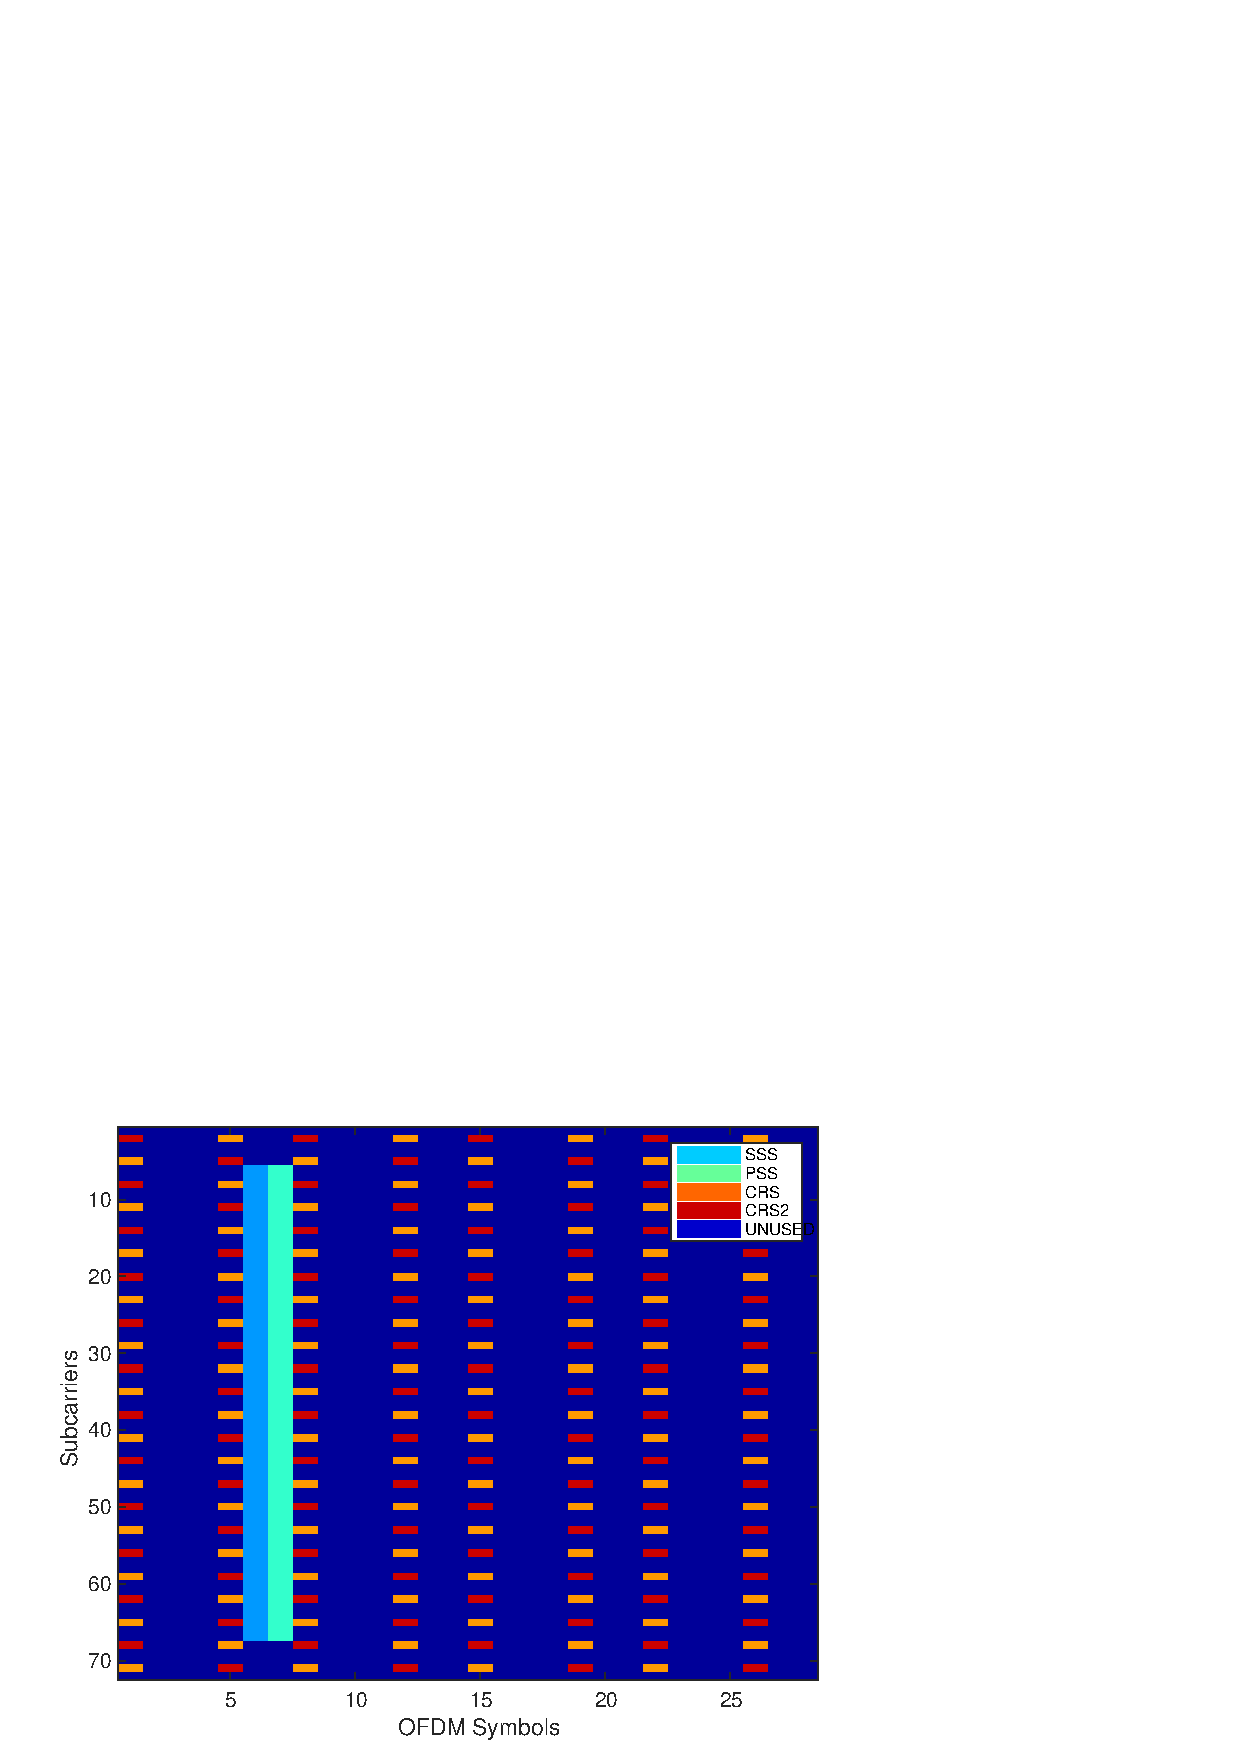
\includegraphics[width=10cm]{images/FrameLegend.png}
        \caption{Resource Block Grid for 2 sub frames}
        \label{fig:RBSignals}
    \end{center}
\end{figure}

One of the disadvantages of using OFDM in the physical layer is the high peak to average power ratio (PAPR) of the signal. High PAPR translates to high fidelity requirements of power amplifiers on the transmitter side. It also induces non-linear distortions to the signal \cite{rohling}. To ensure that the PAPR of the signal is as low as it can be, random QPSK symbols are transmitted on the unused slots instead of 0s.

\subsection{Reception}

For the LTE receiver processing a USRP with 2 antennas acquires the RF data from both ports and processes the data in the FPGA in real time. The data requested by the host is then forwarded to it using the high speed PCIe interface. A more in depth explaination of the receiver processing is explained in Chapter \ref{ch:ExSetup}.

The channel estimation data is forwarded from the FPGA IQ processing engine to the host which is then logged to a TDMS file (NI propriotory format) and post processed to extract samples for the purpose of the experiments. The main steps of the DL receiver processing once enough samples have been captured are the following.


\subsubsection{Carrier Offset Estimation and Correction}
OFDM is extremely senstive to frequency shifts in the received signal. In the case that the receiver or transmitter center frequency clock was not accurate enough, the frequency shift needs to be estimated and corrected. This is the very first step before processing the baseband waveform.

\subsubsection{Frame synchronisation}
As mentioned in Section \ref{LTEFrame} the synchronisation is a very important part of knowing where the LTE frame begins. This is done by correlating the received signal with the known Zadoff Chu Sequence and to look for the peak. Figure \ref{fig:PSSCorr} shows an example correlation of a Zadoff Chu sequence and a received signal containing 307200 samples in total amounting to 2 frames of a 10\si{\mega\hertz} Bandwidth LTE signal. 4 peaks are to be expected here as there are 2 frames, each containing 2 PSS sequences.

\begin{figure}[H]
    \begin{center}
        \includegraphics[width=9cm]{images/PSSCorrelation.jpg}
        \caption{PSS Correlation}
        \label{fig:PSSCorr}
    \end{center}
\end{figure}

\subsubsection{Channel Estimation}

Once the frame has been demodulated and the 2D OFDM grid has been obtained, the channel can be estimated based on the original pilot symbols structure known to the receiver, hence the phase and amplitude of the particular sub carrier can be obtained. A linear interpolator is applied in the frequency axis to interpolate the channel estimate from 200 subcarriers to 1200 subcarriers(for a full bandwidth system) and a zero order hold is used in the time axis until the next pilot symbol in the time domain is encountered. The details are explained in the Chapter \ref{ch:ChEst}.


\subsection{Antenna}
The analog time domain signal is transmitted from the USRP (Section \ref{sec:USRP}) over the air using a Triband antenna. For the setup an omni directional Antenna from NI capable of transmitting and receiving around frequencies of 144, 400 or 1200 \si{\mega\hertz} is used for the transmitter and receiver as shown in Figure \ref{fig:USRPAnt}.

\begin{figure}[H]
    \begin{center}
        \includegraphics[width=7cm]{images/vert400.jpg}
        \caption{Narrowband Omnidirectional Antenna used for transmitting and receiving the LTE Signals}
        \label{fig:USRPAnt}
    \end{center}
\end{figure}

\chapter{Channel Estimation}
\label{ch:ChEst}

LTE was chosen as the standard to use here as it is very mature and has readily available MATLAB/Labview based implementation. In the case of this thesis the aim is not to reinvent standard by redesigning pilot symbol placements. Instead existing standards were used in order to collect experimental data. This reduces design time and focusses more on the issue at hand which is channel estimation data of a MIMO Channel.

\section{OFDM}\label{sec:OFDM}
LTE is based on OFDMA in the physical layer which is a multi carrier communication scheme \cite{FazelKaiser}. As the name suggests OFDM uses orthogonal sub carriers from an orthonormal system to form the basis for independent data streams. For band limited transmission systems with finite access time per channel use the dimension of the parallel data stream is given by the equation \ref{eq:BandLim}  \cite{UtschickOFDM}.

        \begin{equation} \label{eq:BandLim}
            N = BT
        \end{equation}

        \begin{table}[H]
            \begin{center}
                \begin{tabular}{|c|l|}
                    \hline
                    Parameter& Description\\ \hline
                    $N$& Dimension of system \\ \hline
                    $B$& Signal Bandwidth \\ \hline
                    $T$& Channel access time \\
                    \hline
                \end{tabular}
                \caption{}
                \label{tab:BandLimTrans}
            \end{center}
        \end{table}

The orthonormal basis function can be mathematically modelled as the equation \ref{eq:OFDM} \cite{UtschickOFDM}.

        \begin{equation} \label{eq:OFDM}
            \begin{split}
                \psi_{b,q} = p_{T_{b}}(t)exp(j2{\pi}q{\frac{t}{T}}) \\
                p_{T_{b}}(t) = \left\{
                    \begin{matrix}
                        1; & t \in T_b \\
                        0; & otherwise \\
                    \end{matrix}\right.
            \end{split}
        \end{equation}

        \begin{table}[H]
            \begin{center}
                \begin{tabular}{|c|l|}
                    \hline
                    Parameter& Description\\ \hline
                    $\psi_{b,q}$& normalized orthogonal basis functions\\ \hline
                    $b$& channel access slot\\ \hline
                    $q$& sub carrier index\\ \hline
                    $T$& channel access time \\ \hline
                    $T_{b}$& $ t | bT \leq t < (b + 1)T \subset \mathbb{R}$ \\ \hline
                \end{tabular}
                \caption{Parameter definitions for OFDM Definition}
                \label{tab:OFDMParam}
            \end{center}
        \end{table}


        The transmitted data can hence be modelled as the following
        \begin{equation} \label{eq:TxDataMath}
            x_b(t) = \sum_{q=0}^{N-1}\underbrace{X_{b,q}}_\text{data} \psi_{b,q}(t)
        \end{equation}

        For a given ideal AWGN Channel, where there is no delay spread or multipath propogation, the corresponding received data is modelled as
        \begin{equation} \label{eq:RxDataMathIdeal}
            y_b(t) = \sum_{q=0}^{N-1}x_b(t) \psi_{b,q}(t) +\eta_b(t)
        \end{equation}
        where $\eta_b(t)$ is the additive noise

        The demodulation is based on the same set of orthonormal basis vectors that as the receiver, hence we have
        \begin{align*} \label{eq:InnerProductRxIdeal}
            \hat{x}_{b,q} = \langle y,\psi_{b,q}(t)\rangle + \langle\eta_{b},\psi_{b,q}(t)\rangle = x_{b,q}(t) + \eta_{b,q} & & & \forall q = 1,...,N \\
        \end{align*}


\section{MIMO Channel Estimation}\label{sec:MIMO}

\subsection{Maximum Ratio Combiner}\label{ssec:Simple}
\subsection{Zero Forcing}\label{ssec:ZF}
\subsection{MMSE}\label{ssec:MMSE}


\chapter{Potential Hardware Setups}
\label{ch:PotenHWSetup}

Measurements of MIMO channel can be achieved in multiple methods. This chapter discusses some of the potential approaches which were implemented and elaborates each of their advantages and disadvantages.

\section{Software Defined Radios USRP}\label{sec:USRP}

USRP is a Software Defined Radio (SDR) designed by National Instruments that enables quick prototyping of different wireless applications. It is aimed at anyone from hobbists, research labs, universities, etc... or anyone interested in evaluating custom algorithms. The SDR used here is a USRP2940 specifications of which are described in Table \ref{tb:USRP}

\begin{table}[H]
    \begin{center}
        \begin{tabular}{|l|c|}
        \hline
            Model                   & USRP2940          \\ \hline
            Baseband Bandwidth      & 40MHz             \\ \hline
            RF-Operating Frequency  & 50MHz-2200MHz     \\ \hline
            FPGA                    & Kintex-7 410T     \\ \hline
            No of Transmitters      & 2                 \\ \hline
            No of Receivers         & 2                 \\ \hline
            Connectivity            & MXIe, Ethernet    \\ \hline
            Oscillator              & Internal Crystal  \\ \hline
            ADC/DAC                 & 14 (For Rx)/16 (For Tx) bit         \\ \hline
            Frequency Accuracy      & 2.5 ppm           \\ \hline
            Maximum Power Output    & 20dBm             \\ \hline
            Maximum I/Q Sample Rate & 200MHz            \\ \hline
        \end{tabular}
    \end{center}
    \caption{USRP2940 SDR Product details}
    \label{tb:USRP}
\end{table}

\section{MIMO Application Framework (MIMO AFW)}\label{sec:MIMOAFW}
MIMO Application Framework is a Software developed by National Instruments, that offers a comprehensive plug and play MIMO setup. This setup requires a host of additional hardware which are required for the functioning of the MIMO AFW. \cite{MIMOAFWGettingStarted}
\begin{table}[H]
    \begin{center}
        \begin{tabular}{|l|l|}
        \hline
            \textbf{Part Number} & \textbf{Description}          \\ \hline
            USRP-2940            & SDR                           \\ \hline
            PXIe-7976            & FPGA Module for FlexRIO       \\ \hline
            CDA-2990             & Clock Distribution Device     \\ \hline
            CPS-8910             & Switch Device for PCI Express \\ \hline
            PXIe-6674T           & Synchronization Module        \\ \hline
            PXIe-1085            & Chassis                       \\ \hline
            PXIe-8135            & Controller                    \\ \hline
        \end{tabular}
    \end{center}
    \caption{Additional Hardware for required for MIMO AFW to function}
    \label{tb:MIMOAFWPartsList}
\end{table}

\subsection{USRP 2940}\label{MIMOAFWUSRP}
As mentioned in Section \ref{sec:USRP}, this is the backbone of the architecture. The Software defined radio (USRP2940) is used as an air interface for over the air transmission. There are host of other options that can be used here instead of the USRP2940. Table \ref{} lists the alternatives with an overview of the functionality of each of the parts.

    %\clearpage% Flush earlier floats (otherwise order might not be correct)
    %\thispagestyle{empty}% empty page style (?)
    %\begin{landscape}% Landscape page
        %\begin{table}[!htb]
            \begin{sidewaystable}[htp]
                \begin{center}
            %\resizebox{\textwidth}{!}{
                \begin{tabular}{|l|l|l|c|c|c|c|c|}
                \hline
                \textbf{Model} & \textbf{\begin{tabular}[c]{@{}c@{}}RF-Frequency\\ Range\end{tabular}} & \textbf{\begin{tabular}[c]{@{}c@{}}RF-Frontend\\ Bandwidth\end{tabular}} & \textbf{FPGA} & \textbf{Inputs} & \textbf{Outputs} & \textbf{Communication} & \textbf{GPS Osillator} \\ \hline
                USRP-2940      & 50 MHz - 2.2 GHz            & 40 MHz                                & Kintex-7 410T & 2               & 2                & MXIe Ethernet          & No                     \\ \hline
                USRP-2940      & 50 MHz – 2.2 GHz            & 120 MHz                               & Kintex-7 410T & 2               & 2                & MXIe Ethernet          & No                     \\ \hline
                USRP-2942      & 400 MHz - 4.4 GHz           & 40 MHz                                & Kintex-7 410T & 2               & 2                & MXIe Ethernet          & No                     \\ \hline
                USRP-2942      & 400 MHz - 4.4 GHz           & 120 MHz                               & Kintex-7 410T & 2               & 2                & MXIe Ethernet          & No                     \\ \hline
                USRP-2943      & 1.2 GHz - 6 GHz             & 40 MHz                                & Kintex-7 410T & 2               & 2                & MXIe Ethernet          & No                     \\ \hline
                USRP-2943      & 1.2 GHz – 6 GHz             & 120 MHz                               & Kintex-7 410T & 2               & 2                & MXIe Ethernet          & No                     \\ \hline
                USRP-2944      & 10 MHz - 6 GHz              & 160 MHz                               & Kintex-7 410T & 2               & 2                & MXIe Ethernet          & No                     \\ \hline
                USRP-2945      & 10 MHz - 6 GHz              & 80 MHz                                & Kintex-7 410T & 4               & 0                & MXIe Ethernet          & No                     \\ \hline
                USRP-2950      & 50 MHz - 2.2 GHz            & 40 MHz                                & Kintex-7 410T & 2               & 2                & MXIe Ethernet          & Yes                    \\ \hline
                USRP-2950      & 50 MHz - 2.2 GHz            & 120 MHz                               & Kintex-7 410T & 2               & 2                & MXIe Ethernet          & Yes                    \\ \hline
                USRP-2952      & 400 MHz - 4.4 GHz           & 40 MHz                                & Kintex-7 410T & 2               & 2                & MXIe Ethernet          & Yes                    \\ \hline
                USRP-2952      & 400 MHz - 4.4 GHz           & 120 MHz                               & Kintex-7 410T & 2               & 2                & MXIe Ethernet          & Yes                    \\ \hline
                USRP-2953      & 1.2 GHz - 6 GHz             & 40 MHz                                & Kintex-7 410T & 2               & 2                & MXIe Ethernet          & Yes                    \\ \hline
                USRP-2953      & 1.2 GHz - 6 GHz             & 120 MHz                               & Kintex-7 410T & 2               & 2                & MXIe Ethernet          & Yes                    \\ \hline
                USRP-2954      & 10 MHz - 6 GHz              & 160 MHz                               & Kintex-7 410T & 2               & 2                & MXIe Ethernet          & Yes                    \\ \hline
                USRP-2955      & 10 MHz - 6 GHz              & 80 MHz                                & Kintex-7 410T & 4               & 0                & MXIe Ethernet          & Yes                    \\ \hline
                \end{tabular}
            %}
            \end{center}
            \caption{List of alternative Software defined radios offered by National Instruments}
            \label{tb:USRPPartsList}
        \end{sidewaystable}
%\end{landscape}
%\clearpage% Flush page


\section{LTE Application Framework}\label{sec:LTEAFW}

LTE Application Framework is a Software that National Instruments designed and offers to set up a LTE setup. This setup requires a host of additional hardware which are required for the functioning of the LTE AFW.

%\begin{figure}[!htb]
%    \centering
%    \includegraphics[width=7cm]{../ReportImages/TxPwrSetup.png}
%    \caption{Setup for measuring the transmit power}%
%    \label{fig:TxPwrSetup}%
%\end{figure}


\chapter{Experimantal Setup}
\label{ch:ExSetup}

Chapter \ref{ch:PotenHWSetup} discussed the possible options to implement a MIMO setup. The first option (Section \ref{sec:USRP}) was not viable due to technical limitations as it is described in Appendix \ref{sec:USRPSync}.

The second option (Section \ref{sec:MIMOAFW}) was financially unfeasible as the additional hardware for the modular MIMO set was to cost over €100.000. The only viable option was to use the LTE AFW with a MIMO Extension, although limited to a 2x2 MIMO system, was sufficient in this case.

\section{LTE Application Framework MIMO Extension}\label{sec:LTEAFWMIMOExt}

LTE AFW is a SISO LTE Release 10 implementation, where as LTE AFW 2x2 MIMO Extension was developed internally by NI as a plugin to the SISO framework to demonstrate a proof of concept for their MIMO Application Framework product. The main goal of LTE 2x2 MIMO Extension was to demonstrate a functioning 2x2 MIMO System. It is implemented for \textbf{DL only}. The software is not readily available for customers to purchase, but it was given to MSV as a workaround for the MIMO implementation.

For the implementation of the LTE AFW MIMO Extension as outlined in Chapter \ref{sec:LTEAFW} the equipment required is minimal. A set of 2 USRPs, one acting as a UE (Receiver) and the other acting as a Base Station (eNodeB) completes the transceiver chain and the Host PC does the graphing, data visualisation, user data communications and device setup. Figure \ref{fig:LTEAFWHWSetup} illustrates the simple HW connections required to make the device communicate with the host. For details on the part descriptions refer to Section \ref{ssec:LTEAFWHW}.

\begin{figure}[!htb]
    \centering
    \includegraphics[width=11cm]{images/MIMOSetUpArrangement.png}
    \caption{Overview of the LTE 2x2 MIMOHW Connections}
    \label{fig:LTEAFWHWSetup}
\end{figure}


\subsection{LTE AFW MIMO Extension Architecture}\label{ssec:LTEAFWArch}

\begin{figure}[!htb]
    \centering
    \includegraphics[width=\linewidth]{images/LTEAFW2x2ExtBlockDiagram.png}
    \caption{Overview of a 2 device Tx-Rx setup as intended in the final implementation}
    \label{fig:LTEAFW2DeviceOverview}
\end{figure}

Figure %s \ref{fig:LTEAFWExtArch} and 
\ref{fig:LTEAFW2DeviceOverview} shows the block diagram of the system in the DL, eNodeB and UE operation modes. Data streams that require high data rates for data transfer between host and FPGA are implemented as DMA FIFOs. These streams include the payload and UL data from host to FPGA and the received PDSCH/PUSCH transport blocks from FPGA to host. In-phase/quadrature (I/Q) samples for constellation and spectrum display as well as the channel estimation (\textbf{ONLY} \textit{h11} and \textit{h22}) values are also transferred from FPGA to host using DMA FIFOs. Further status information is transferred to the host by reading the indicator values \cite{LTEAFWManual}. As it can be seen both RX and TX components are implemented in the Host Software as well as in the FPGA Hardware. Hence the same application can be used as an \textit{eNodeB} as well as \textit{UE}. The \textit{eNodeB} mode uses the DL TX processing units and \textit{UE} uses the DL RX processing units which are explained in Section \ref{ssec:LTEAFWFPGA}. The following lists the various processing blocks in the application and a brief description of the corresponding tasks of each of the modules.

\begin{itemize}
    \item \textbf{UDP read} -
        Reads data, provided by an external application, from a UDP socket. The data is used as payload data in the transport block (TB). This data is then encoded and modulated as an LTE DL signal by the downlink transmitter (DL TX PHY).
    \item \textbf{UDP write} -
        Writes the payload data, which was received and decoded from the LTE DL signal by the downlink receiver (DL RX PHY), to a UDP socket. The data can then be read by an external application.
    \item \textbf{MCS and MIMO Flag} -
        Creates a cluster including the required information for the downlink control information (DCI) message such as the modulation and coding scheme (MCS) and the MIMO flag. The MIMO flag is a control that is used to activate MIMO or SISO in the eNodeB.
    \item \textbf{DEMUX} -
        A demultiplexer is used to split the data stream to Data Stream 1 and Data Stream 2 if the transmitter is configured to use both RF chains for TX. 
    \item \textbf{Data Buffer} -
        Two buffers are used to store data coming from the Payload H2T FIFO into two local FIFOs for TX chain 1 and TX chain 2. In the RX mode, two buffers are used to store the received data coming from the synchronization module to synchronize the signal processing in RX chain1 and RX chain 2.
    \item \textbf{MAC TX} -
        A simple MAC implementation that adds a header to the TB containing the number of payload bytes. The header is followed by the payload bytes, and the remaining bits of the TB are filled with padding bits.
    \item \textbf{DL TX PHY} -
        Physical layer (PHY) of the downlink (DL) transmitter (TX). Encodes the physical channels and creates the LTE downlink signal as digital baseband I/Q data. This code includes encoding of the control channel (PDCCH), encoding of the data channel (PDSCH), resource mapping, and orthogonal frequency-division multiplexing (OFDM) modulation. The white paper Labview communications LTE Application Framework 19.5\cite{LTEAFWManual} has the details of the implementation of the TX Bit Processing and IQ Signal Processing.
    \item \textbf{Sync} -
        The primary synchronization sequence (PSS) is used for synchronization. The synchronization is done using the received signal on RF0/RX2. The synchronization results such as frame alignment and frequency offsets estimation (integral and fractional) are used to adjust the received signals on both ports RF0/RX2 and RF1/RX2.
    \item \textbf{DL RX PHY} -
        Physical layer (PHY) of the downlink (DL) receiver (RX). Demodulates the LTE downlink signal and decodes the physical channels, OFDM demodulation, resource demapping, MIMO channel estimation and MIMO equalization, decoding of the control channel (PDCCH), and decoding of the data channel (shared channel, PDSCH). For MIMO equalization, three algorithms have been implemented namely: simple algorithm, minimum mean squared error (MMSE), and zero-forcing (ZF). The simple algorithm means that the inverse of the estimated channel parameters is used directly in the equalizer. There is also an option of disabling the equalization using a switch to get raw data.
    \item \textbf{MUX} -
        A multiplexer is used to combine the received data from both RX chains to be transmitted to the host.
    \item \textbf{MAC RX} -
        Disassembles the TB and extracts the payload bytes.
    \item \textbf{SINR calculation} -
        Calculates the signal-to-interference-noise-ratio (SINR) based on the channel estimation that was used for PDSCH decoding. Channel estimation is either based on cell-specific reference signals (CRS), or on UE-specific reference signals (UERS).
    \item \textbf{RF} -
        In the transmit path, it performs digital up conversion (DUC), RF impairments correction, and writes the transmit data to the RF. In the receive path, it reads the received data from the RF, performs digital down conversion (DDC) and performs RF impairments correction.
\end{itemize}

%\begin{figure}[H]
%    \centering
%    \includegraphics[width=11.5cm]{images/LTEAFWExtArch.png}
%    \caption{Overview of the LTE 2x2 MIMO Architecture and the HW/SW design split}
%    \label{fig:LTEAFWExtArch}
%\end{figure}

\subsection{LTE AFW Host Software}\label{ssec:LTEAFWHostSW}
The LTE AFW 2x2 MIMO application uses a UDP stream to transfer data between the host and the device or vice versa. Figure \ref{fig:UDPDataTransfer} shows the end to end data flow starting from the host, going through the data FIFOs set up in the FPGAs and back to the host again where the received data is displayed.

\begin{figure}[H]
    \centering
    \includegraphics[width=8cm]{images/UDPDataTransfer.png}
    \caption{UDP Host-Device Data transfer}
    \label{fig:UDPDataTransfer}
\end{figure}

\subsubsection{Host Software Modifications}\label{ssec:LTEAFWHostSWMods}
The host software was heavily modified for the following reasons

\begin{itemize}
    \item The version of the software given to MSV by NI was intended for an older version \textit{LabVIEW Communication System Design Suite 2.0} which was only supported for all OS releases until Windows 8.1/7 64-bit.

    \item The FPGA source was not issued to MSV instead a pre compiled FPGA bit file was delivered, but this corresponded to the \textbf{old} version namely \textit{Labview Communications System Design Suite 2.0}.

    \item The project was not forwards compatible with the latest version of the Labview Communications System Design Suite.
\end{itemize}

As a result of the above mentioned point and to guarentee future compatibility, the project had to be ported to the latest version of \textit{LabVIEW Communication System Design Suite 4.0}, which was renamed as \textit{Labview NXG 4.0}. Missing dependencies had to be manually included and many driver related functionalities had to be modified as the newer version had a different driver implementation compared to the older version.

\subsubsection{DL Receiver}\label{ssec:LTEAFWRXOptions}

The DL Receiver implements the end to end receiver chain from receiving the raw data from the RF Frontend to the OFDM processing, demodulation and LTE processing steps. Most of the complex resource intensive data processing is done onboard the FPGA as mentioned in Section \ref{ssec:LTEAFWFPGA}. Certain parameters of the receiver can be manually configured according to user specifications. The chosen settings for this experiment are listed in Table \ref{tab:RXUSRPParam}.

\begin{table}[H]
    \begin{center}
        \begin{tabular}{|l|l|}
            \hline
            \textbf{Parameter}                                                          & \textbf{Value} \\ \hline
            Center Frequency                                                            & 1.2\si{\giga\hertz}         \\ \hline
            Transmit IP Address	                                                        &
127.0.0.1      \\ \hline
            UDP Receive Port                                                            & 60000          \\ \hline
            \begin{tabular}[c]{@{}l@{}}Receiver RX Antenna \\ Port On USRP\end{tabular} & RX2/RF1        \\ \hline
                Cell ID                                                                     & 0              \\ \hline
                LTE Duplexing Mode                                                          & FDD            \\ \hline
                Manual Receiver Gain                                                        & 20\si{\dB}           \\ \hline
        \end{tabular}
        \caption{Receiver USRP Parameters Setup}
        \label{tab:RXUSRPParam}
    \end{center}
\end{table}

The DL RX (UE) mode screens are shown in Figures \ref{fig:DLRXScreen} and \ref{fig:DLRXAdvScreen}.

\begin{figure}[H]
    \centering
    \includegraphics[width=\linewidth]{images/SISORXEdited.png}
    \caption{A Screencapture of the DL RX(UE) side application window}
    \label{fig:DLRXScreen}
\end{figure}

\begin{figure}[H]
    \centering
    \includegraphics[width=\linewidth]{images/SISORXADVEdited.png}
    \caption{A Screencapture of the DL RX(UE) Advanced Options in the application window}
    \label{fig:DLRXAdvScreen}
\end{figure}

Table \ref{tab:RXUSRPParamDesc} describes the various graphs and indicators shown on the RX screen of the application.

\begin{landscape}
    % Please add the following required packages to your document preamble:
    % \usepackage[normalem]{ulem}
    % \useunder{\uline}{\ul}{}
    \begin{table}[]
        \begin{tabular}{|l|p{14cm}|}
            \hline
            \textbf{Indicator}         & \textbf{Description}                                                                                                                                                                                                                                                                  \\ \hline
            MIMO flag                  & Activates the eNodeB to run in MIMO setup. The MIMO flag is included in the DCI message to be deciphered at the RX part of UE.                                                                                                                                                        \\ \hline
            Equalizer Type             & Configures the algorithm that is used for equalization. The enumeration contains the following values: MMSE, ZF, and Simple.                                                                                                                                                          \\ \hline
            Sigma                      & Selects the scaling factor that is used in the MMSE channel equalizer.                                                                                                                                                                                                                \\ \hline
            MIMO Selector AP0          & Determines the PDSCH Constellation of AP0 that has been derived from SISO equalizer or MIMO equalizer.                                                                                                                                                                                \\ \hline
            eNB TX Power Spectrum AP0  & Shows the power spectrum of the DL TX baseband signal transferred to the RF0/TX1.                                                                                                                                                                                                     \\ \hline
            eNB TX Power Spectrum AP1  & Shows the power spectrum of the DL TX baseband signal transferred to the RF1/TX1.                                                                                                                                                                                                     \\ \hline
            UE RX Power spectrum AP0   & Shows the power spectrum of the DL RX baseband signal received from RF0/RX2.  If synchronization is successful based on the received signal from RX1 (RF0/RX2), frame timing and frequency offset correction are applied on the received signals from both ports RF0/RX2 and RF1/RX2. \\ \hline
            UE RX Power spectrum AP1   & Shows the power spectrum of the DL RX baseband signal received from RF1/RX2.                                                                                                                                                                                                          \\ \hline
            PDSCH Constellation of AP0 & Constellation of RX IQ samples of AP0 allocated for PDSCH transmission after SISO or MIMO equalization. Only samples for the configured OFDM Symbol-Nr (PDSCH) are displayed.                                                                                                         \\ \hline
            PDSCH Constellation of AP1 & Constellation of RX IQ samples of AP1 allocated for PDSCH transmission after MIMO equalization. Only samples for the configured OFDM Symbol-Nr (PDSCH) are displayed.                                                                                                                 \\ \hline
            Channel Estimation of AP0  & Graphical representation of the normalized channel amplitude and phase estimated based on the cell specific reference signals of AP0                                                                                                                                                  \\ \hline
            Channel Estimation of AP1  & Graphical representation of the normalized channel amplitude and phase estimated on the cell specific reference signals of AP1.                                                                                                                                                       \\ \hline
        \end{tabular}
        \caption{Receiver USRP indicators description}
        \label{tab:RXUSRPParamDesc}
    \end{table}
\end{landscape}

\subsubsection{DL Transmitter}\label{ssec:LTEAFWTXOptions}

\subsection{LTE AFW FPGA}\label{ssec:LTEAFWFPGA}
LTE has demanding and resource intensive processing requirements and in the application framework, the processing blocks for the DL and UL TX and RX are implemented directly on the FPGA. They exchange the baseband data with the RF interface using target-scoped FIFOs. The processing on the FPGA has advantages because it provides lower latency and therefore enables real-time physical layer processing. The following section describe the steps involved in the DL TX and DL RX processing done on the FPGA.

\subsubsection{DL TX IQ Processing}\label{sssec:DLTXIQProc}

\begin{figure}[!htb]
    \centering
    \includegraphics[width=\linewidth]{images/DLFPGATXImpl.png}
    \caption{Simplified implementation of the DL TX processing block of the FPGA}
    \label{fig:LTEAFWFPGADLTXProc}
\end{figure}

\subsubsection{DL RX IQ Processing}\label{sssec:DLRXIQProc}

This module reads the radio-frame aligned signal in time domain and outputs the channel-equalized subcarriers that are associated to the physical channels. As shown in Figure \ref{fig:LTEAFWFPGADLRXProc}, it includes the following functional blocks

\begin{figure}[!htb]
    \centering
    \includegraphics[width=\linewidth]{images/DLFPGARXImpl.png}
    \caption{Simplified implementation of the DL RX processing block of the FPGA}
    \label{fig:LTEAFWFPGADLRXProc}
\end{figure}

\begin{itemize}
    \item \textbf{Radio Frame Synchronization} -
        Synchronization is vital for the time alignment of the Frames as OFDM is extreamly time sensitive. CFO (Carrier Frequency Offset) correction is important to correct for any error/inaccuracies in the local oscilators. This could inadvertently move the frequency grid up or down based on the offset. Synchronization and CFO compensation are achieved by continuous measurement of both an autocorrelation and a cross correlation. LTE signals contain a PSS, which is detected by two finite impulse response (FIR) filters (real and imaginary part) that calculate the cross correlation. This operation is executed on a reduced sample rate of 1.92 MS/s, which is the result of a decimation by 16. For each radio frame, the cross correlation peak is detected. To avoid misdetection, a validation unit checks that the peak amplitude is eight times higher than the average energy of the cross correlation. Additionally, three consecutive peaks are required, and the peak position may not drift more than five samples.
    \item \textbf{CP removal} -
        An internal FIFO is used to decouple the incoming samples from the rest of the processing chain. The throttle control module waits until enough samples for one complete OFDM symbol (FFT size + CP) are available before it passes them as a consecutive stream to the next modules. The CP removal removes the valid flag from the samples belonging to the cyclic prefix. The 2,048 remaining samples are sent to a Xilinx FFT. For a full 20 \si{\mega\hertz} BW LTE system the number of samples in a subframe is 2048 plus the CP samples that are added during the TX process. Once the CP is removed the remaining 2048 Samples are forwarded onto the FFT Conversion module.
    \item \textbf{FFT Conversion} -
        The output of the FFT are 2048 the subcarriers in frequency domain.
    \item \textbf{Resource demapping} -
        The resource demapper selects the 1200 allocated subcarriers by removing the surrounding whitespace and the DC carrier in the center. Then it generates the timing information for each sample and the resource grid by marking each sample for its corresponding channel by using a Boolean cluster. The resource mapping is based on a fixed frame structure configuration described in the LTE specifications. All subsequent modules use this Boolean cluster with elements for each LTE channel to determine if this sample is relevant.
    \item \textbf{CRS based channel estimation and equalization} -
        The FFT output data is fed into two separate channel estimation blocks running in parallel. The first channel estimation is based on the CRS. The channel estimate values are calculated by conjugate complex multiplications. A linear interpolation is applied in frequency domain between adjacent reference symbols. On the edges of the symbol, the nearest estimated value is replicated (zero order hold). OFDM symbols not containing CRS sequences rely on the last channel estimation (zero order hold in time) as shown in Figure \ref{fig:ChEstInterpolation}
    \item \textbf{UERS based channel estimation and equalization} -
        This signalling scheme is available for use but not actively used in this thesis.
\end{itemize}

\begin{figure}%
    \centering
    \subfloat[Channel Estimation Interpolation over Frequency]{{\includegraphics[width=5cm]{images/ChEstInterpolation.png} }}%
    \qquad
    \subfloat[Channel Estimation Zero order hold over time]{{\includegraphics[width=5cm]{images/ChEstZOH.png} }}%
    \caption{Illustration of channel estimation interpolation over time and frequency}%
    \label{fig:ChEstInterpolation}%
\end{figure}

\section{Application Example}\label{sec:AppEx}
\begin{table}[H]
    \begin{center}
        \begin{tabular}{|c|c|}
            \hline
            \textbf{Coefficient Index} & \textbf{Coefficient Values} \\ \hline
            0                          & 0                           \\ \hline
            1                          & -0.061235467                \\ \hline
            2                          & 0                           \\ \hline
            3                          & 0.306177333                 \\ \hline
            4                          & 0.510116268                 \\ \hline
            5                          & 0.306177333                 \\ \hline
            6                          & 0                           \\ \hline
            7                          & -0.061235467                \\ \hline
            8                          & 0                           \\ \hline
        \end{tabular}
    \end{center}
\end{table}


\chapter{Results}
\label{ch:results}

Over the course of the internship many different parameters had to be determined and set up for the final demo. This chapters documents the results of all the experiments performed as well as the final demo of the working setup.

%\section{Results}\label{sec:Results}
\section{Data Loss}\label{ssec:DataLoss}

Following the data transmission through over the air using LTE AFW, benchmarks were run to check the loss of data over the wireless medium. Tests were run using \textit{iperf} version 2.0.9.


\chapter{Conclusion and Outlook}\label{ch:conOutlook}

\section{FPGA File Port}\label{sec:FPGAChange}
Currently the FPGA Hardware design is where all the data is being received from the RF Front end and processed. This is a pre compiled bit file delivered by NI to work with their version of the LTE AFW Software. To adapt the design to suit the needs of the current research, the FPGA bit file has to be ported to suit our design 

%TODO add photos of the missing dependencies

\section{Experiment with structured Channel}\label{sec:StrucChannel}



%\chapter{Example with Citations}
%\blindtext
%
%\section{Citation and Equation}
%If we write a floating point definition without suffixes$\mathrm{suffixes}\operatorname{suffixes}$ as in $y = \sin(x)$ sin(x), we obtain inline math symbols~\cite{Aldroubi01,Bazaraa06,WeStSh06}.
%\begin{equation}
%\prod_{j=1}^J\sum_{i=1}^\infty \int_{-\infty}^\zeta e^{\xi^2/\nu}d\xi \int_{S^1} \mathcal{R}f_i^j(\omega) d\omega
%\end{equation}
%\begin{equation}
%\left(\frac{\sin(x)}{\pi x} <\leq=\geq>|\|\sim+-\pm \| z^Hz\|\right)\quad \forall \zeta \in R
%\end{equation}%
%
%\blindtext[8]
%
%\section{This is a Section}
%\blindtext[1]
%
%\subsection{This is a Subsection}
%\blindtext[1]
%
%\subsubsection{This is a Subsubsection}
%\blindtext[1]
%
%\paragraph{This is a Paragraph}
%\blindtext[1]
%
%\subparagraph{This is a Subparagraph}
%\blindtext[1]
%
%
%\chapter{Check Text Height}
%\blindtext[40]
%
%\blindmathtrue
%\Blinddocument
%\blinddocument


%--------------------------------------------------------------------------------
% ** Appendix
%
\appendix
\chapter{Antenna Pattern}
\label{ch:AntennaPat}

\section{Transmit Power Measurements}\label{GainDistortion}

\section{Demo}


\chapter{Schematic Octoclock}
\label{ch:HWSchOctoClock}


\chapter{Troubleshooting}
\label{ch:troubleshooting}


\cleardoublepage
% \bibliographystyle{unsrt}
%--------------------------------------------------------------------------------
% ** References 
\bibliographystyle{IEEEtran}
\refstepcounter{chapter}
\addcontentsline{toc}{chapter}{\bibname}
\bibliography{bibfile}

% \cleardoublepage
% \refstepcounter{chapter}
% \addcontentsline{toc}{chapter}{\indexname}
% \printindex
% \end{comment}
\end{document}
